\section{3D Design \& Mechanical Engineering}

\subsection{Enclosure Design Overview}

The BAKO Motors ISS board requires a protective enclosure that shields the PCB from mechanical vibration, dust, and incidental contact with vehicle components, while still providing clear access to all external connectors and sensor cables. The enclosure was designed from scratch as a 3D-printable ABS/PLA part using parametric CAD software, sized to match the ISS board footprint and the connector layout established in the KiCad PCB (Rev.~RECTIFICATION\_2).

The design objectives were:
\begin{itemize}
    \item \textbf{Secure board mounting} — four corner bosses with through-holes accept M3 screws that fasten the PCB directly to the enclosure floor without additional standoffs.
    \item \textbf{Cable egress slots} — rectangular cutouts on two opposing side walls accommodate the vehicle harness connectors (CAN bus J1, power J9, sensor bundles) and the USB programming port without stressing the PCB edge connectors.
    \item \textbf{Open-top access} — the enclosure is a lidded tray; the open-top design allows heat generated by the LM2596S-ADJ switching regulator to dissipate naturally and provides easy PCB removal for re-flashing.
    \item \textbf{Brand identification} --- \textit{SMU-BAKO} and \textit{Senior CSE 2026} text is embossed on the exterior walls to identify the unit during installation.
\end{itemize}

\subsection{CAD Model}

The enclosure geometry was modelled in a parametric CAD environment. The model consists of a single-body rectangular tray with a uniform 2~mm wall thickness, an internal floor that matches the PCB outline, four corner mounting bosses, and two sets of rectangular cutouts on opposing side walls for the wiring harness.

Figures~\ref{fig:case-cad-front} and~\ref{fig:case-cad-side} show the CAD model from two isometric viewpoints, illustrating the cable egress slots and the embossed labelling on the exterior faces.

\begin{figure}[H]
    \centering
    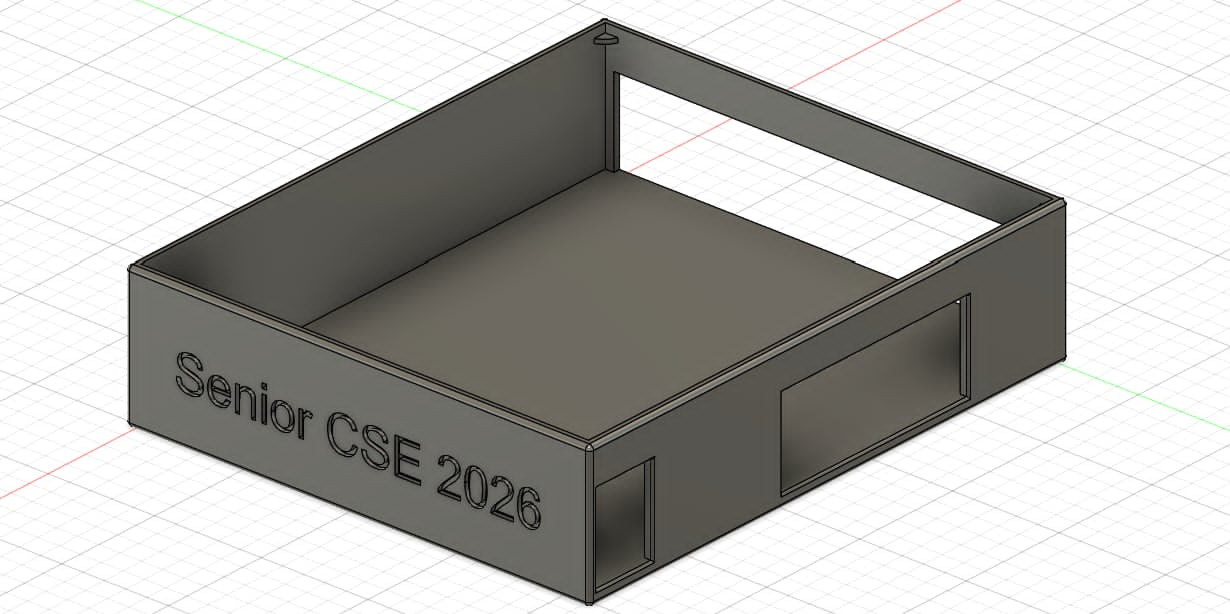
\includegraphics[width=0.82\textwidth]{images/Untitled.jpeg}
    \caption{ISS enclosure CAD model --- isometric front-right view showing the ``Senior CSE 2026'' embossed face and the rectangular connector cutout on the right side wall.}\label{fig:case-cad-front}
\end{figure}

\begin{figure}[H]
    \centering
    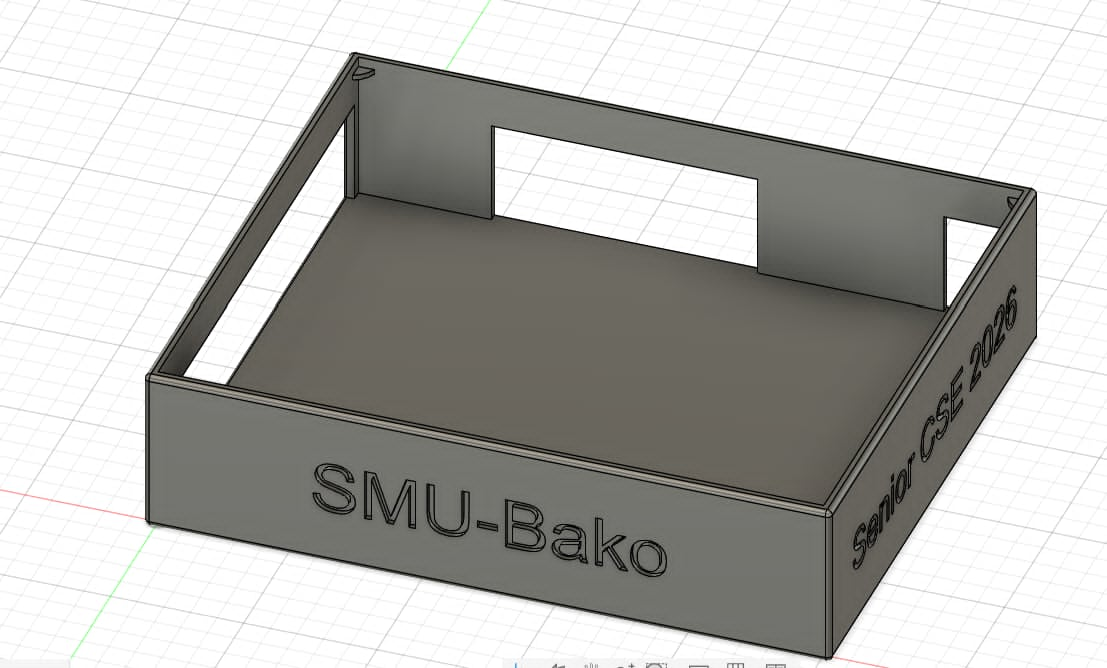
\includegraphics[width=0.82\textwidth]{images/Untitled1.jpeg}
    \caption{ISS enclosure CAD model --- isometric front-left view showing the ``SMU-Bako'' and ``Senior CSE 2026'' embossed faces and the cable egress slots on two walls.}\label{fig:case-cad-side}
\end{figure}

\subsection{3D Print Preparation \& Slicing}

The CAD model was exported as an STL file and imported into \textbf{Bambu Studio} for print preparation. Bambu Studio's slicer was used to orient the part, generate support structures, and configure print parameters for a Bambu Lab printer with a textured PEI plate. The enclosure prints in a single session without post-processing assembly.

Figures~\ref{fig:case-slicer-a},~\ref{fig:case-slicer-b}, and~\ref{fig:case-slicer-c} show the sliced model from three orientations in the Bambu Studio build plate preview, confirming correct orientation (open face up), corner mounting feet visible from all angles, and no unsupported overhangs requiring internal supports.

\begin{figure}[H]
    \centering
    \begin{subfigure}[b]{0.48\textwidth}
        \centering
        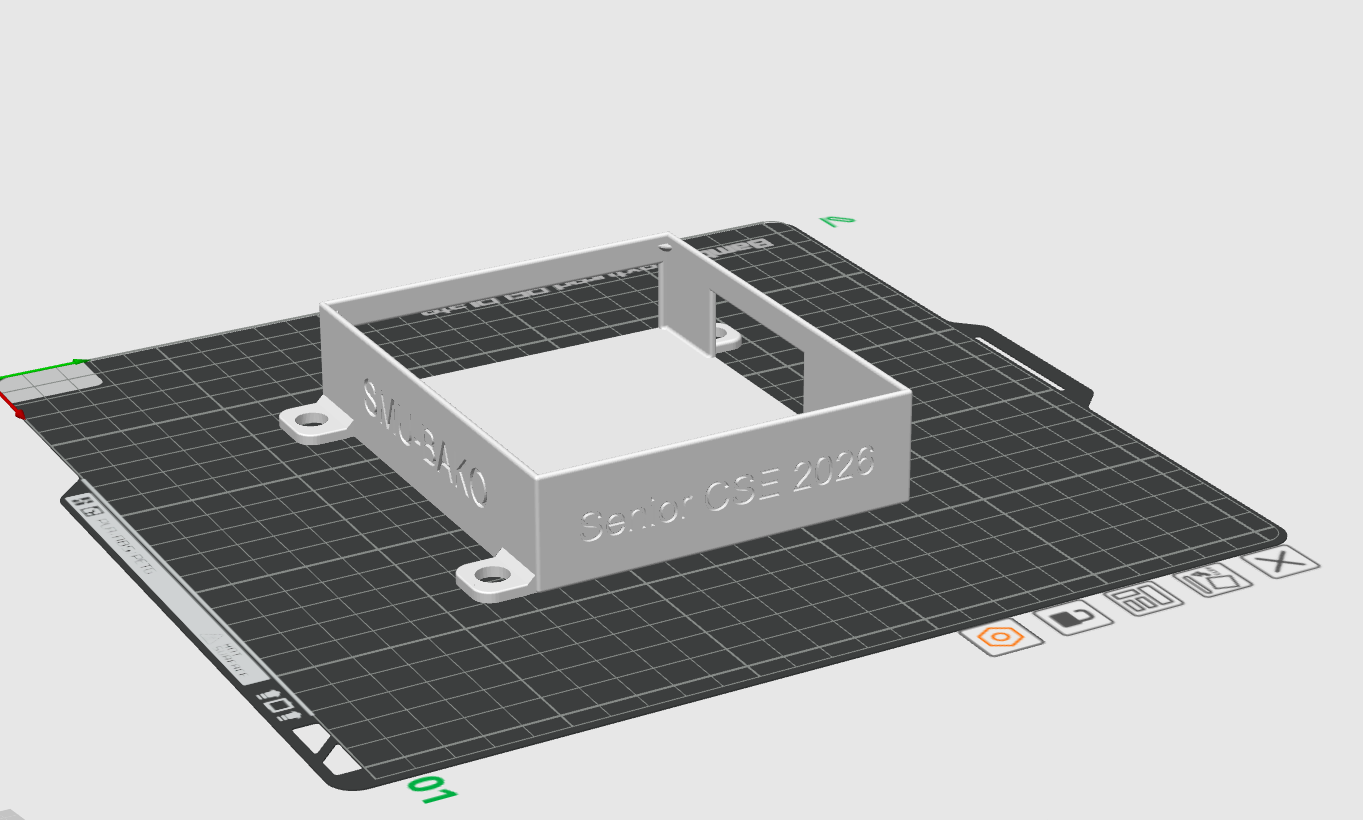
\includegraphics[width=\textwidth]{images/1.PNG}
        \caption{Isometric front-right --- ``SMU-BAKO / Senior CSE 2026'' labelling and mounting corner feet visible.}\label{fig:case-slicer-a}
    \end{subfigure}
    \hfill
    \begin{subfigure}[b]{0.48\textwidth}
        \centering
        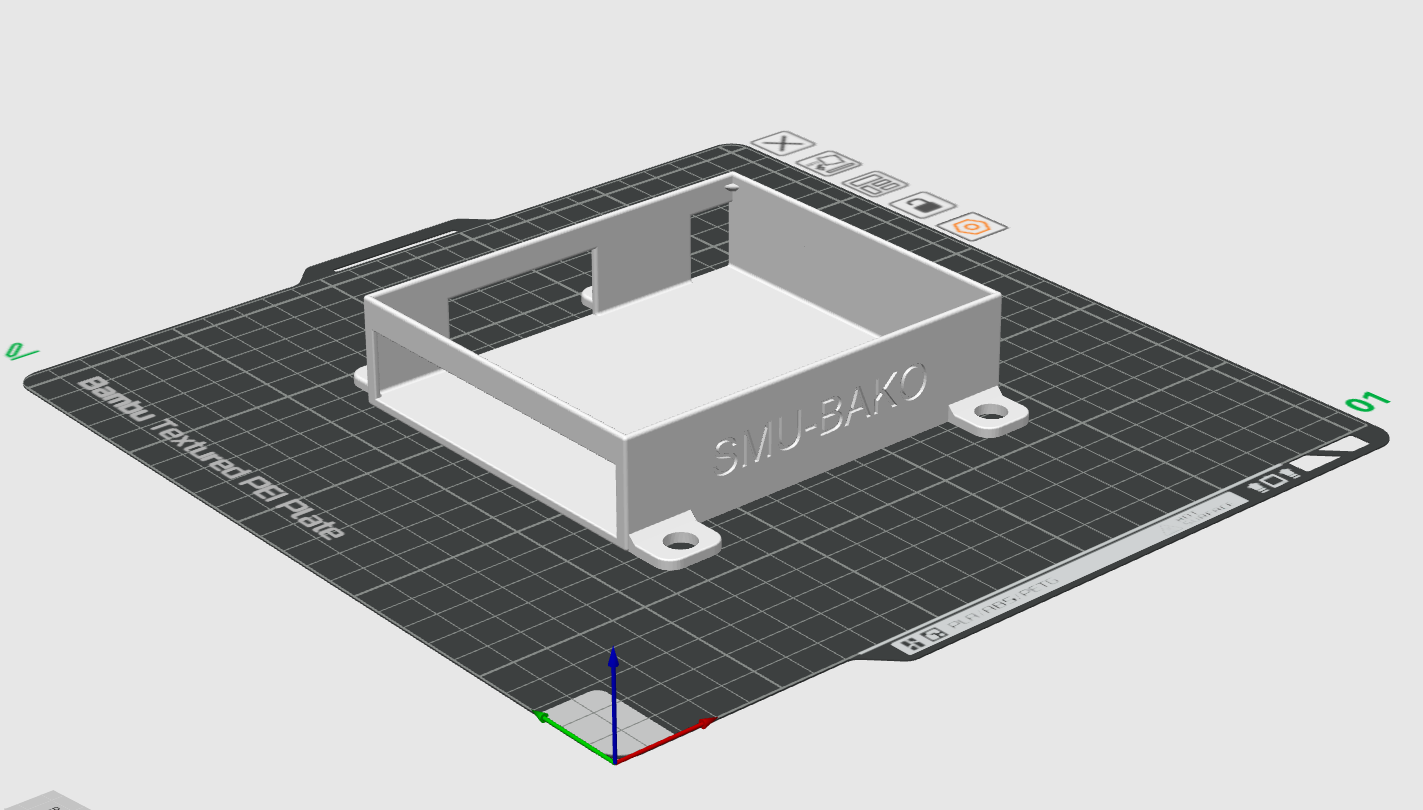
\includegraphics[width=\textwidth]{images/2.PNG}
        \caption{Isometric front-left --- front cable egress slot and open-top orientation confirmed.}\label{fig:case-slicer-b}
    \end{subfigure}

    \vspace{0.5em}

    \begin{subfigure}[b]{0.65\textwidth}
        \centering
        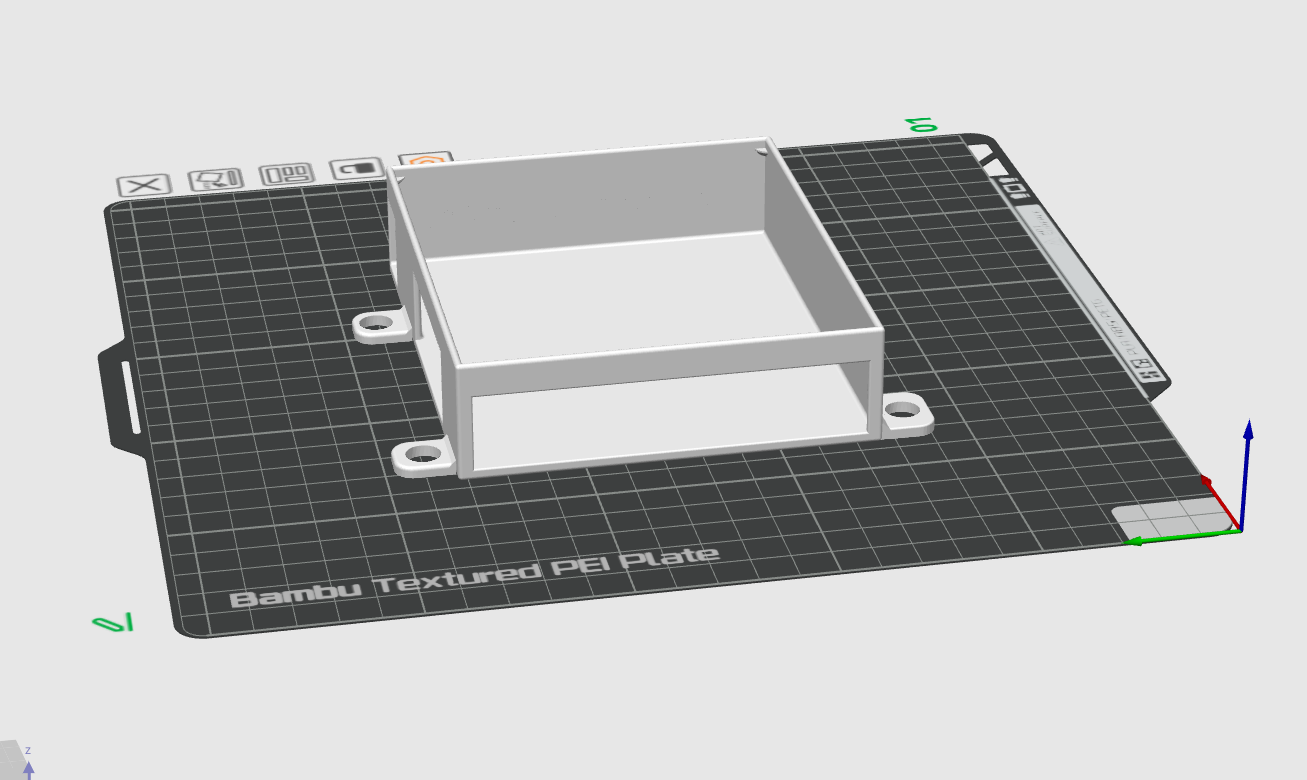
\includegraphics[width=\textwidth]{images/3.PNG}
        \caption{Rear isometric view --- two back-wall cutouts for the vehicle harness and CAN bus connector visible.}\label{fig:case-slicer-c}
    \end{subfigure}
    \caption{Bambu Studio slicer views of the ISS enclosure on the textured PEI build plate, shown from three orientations. The enclosure prints open-face-up with no supports required.}\label{fig:case-slicer-all}
\end{figure}

\subsection{Mechanical Features Summary}

Table~\ref{tab:case-features} summarises the key mechanical parameters of the enclosure as designed.

\begin{table}[H]
\centering
\caption{ISS Enclosure Mechanical Parameters}\label{tab:case-features}
\begin{tabular}{>{\bfseries}p{4.2cm} p{8.5cm}}
\toprule
Parameter & Value \\
\midrule
Design tool        & Parametric CAD (Fusion 360 / equivalent) \\
Slicer             & Bambu Studio \\
Print orientation  & Open face up, flat on build plate \\
Wall thickness     & 2~mm uniform \\
Material           & PLA or PETG (prototype); ABS for vehicle environment \\
Corner mounting    & 4$\times$ M3 boss, 6~mm diameter, through-hole for PCB screws \\
Cable egress slots & 2 side walls; rectangular cutouts sized for JST + screw-terminal connectors \\
Exterior labelling & ``SMU-BAKO'' and ``Senior CSE 2026'' embossed text, 0.5~mm depth \\
Protection rating  & Open-top prototype; IP-rated lid deferred to next revision \\
\bottomrule
\end{tabular}
\end{table}

The enclosure design is production-ready for the prototype phase. A sealed lid with gasket groove and SIM800L antenna pass-through is identified as a short-term development item for field deployment, targeting IP54 ingress protection as noted in the recommendations chapter (Section~\ref{sec:recommendations}).
